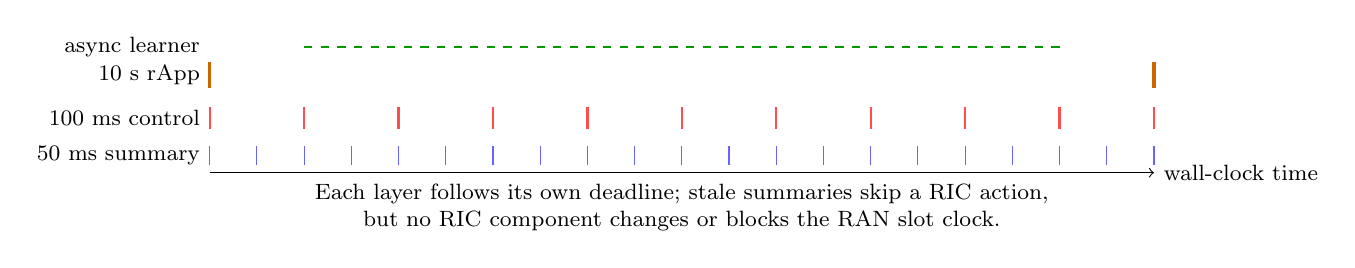
\begin{tikzpicture}[font=\footnotesize,x=0.012cm,y=0.8cm]
\draw[->] (0,0) -- (1000,0) node[right]{wall-clock time};
\foreach \x in {0,50,...,1000} \draw[blue!60] (\x,0.12)--(\x,0.42);
\node[left] at (0,0.28) {50 ms summary};
\foreach \x in {0,100,...,1000} \draw[red!70,thick] (\x,0.7)--(\x,1.05);
\node[left] at (0,0.87) {100 ms control};
\draw[orange!80!black,very thick] (0,1.35)--(0,1.75);
\draw[orange!80!black,very thick] (1000,1.35)--(1000,1.75);
\node[left] at (0,1.55) {10 s rApp};
\draw[green!60!black,thick,dashed] (100,2.0)--(900,2.0);
\node[left] at (0,2.0) {async learner};
\node[align=center] at (500,-0.55) {Each layer follows its own deadline; stale summaries skip a RIC action,\\but no RIC component changes or blocks the RAN slot clock.};
\end{tikzpicture}
